\documentclass[tikz,border=8pt]{standalone}
\usepackage{pgfplots}
\usepgfplotslibrary{groupplots}
\pgfplotsset{compat=1.18}
\begin{document}
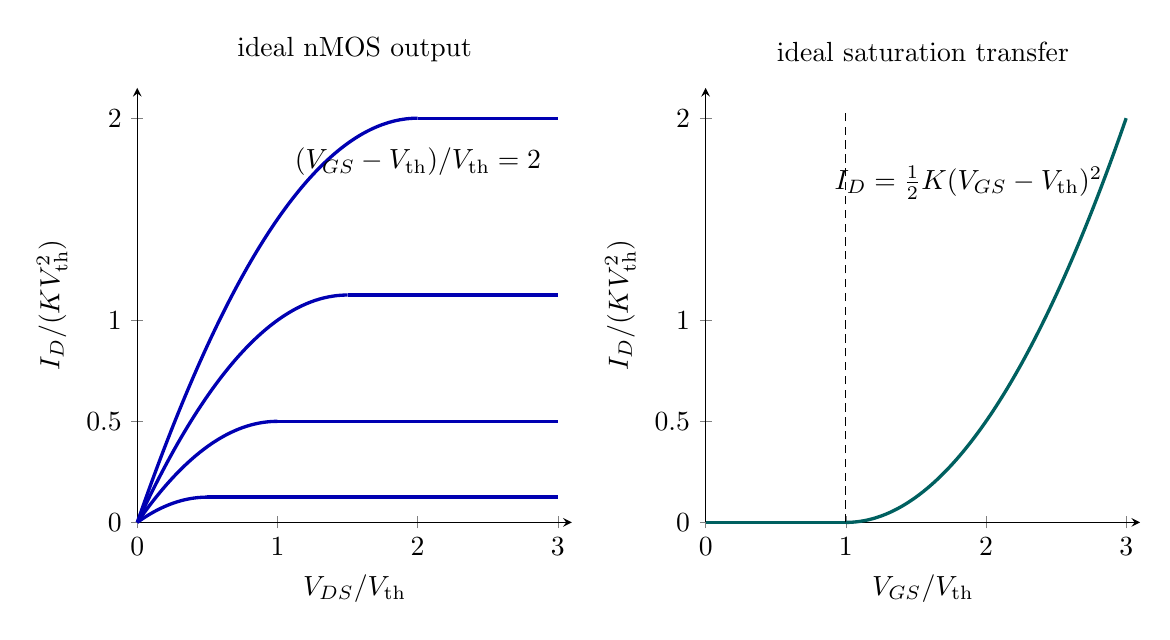
\begin{tikzpicture}
\begin{groupplot}[
  group style={group size=2 by 1,horizontal sep=1.7cm},
  width=7.1cm,height=7.1cm,axis lines=left,clip=false
]
\nextgroupplot[
  title={ideal nMOS output},xmin=0,xmax=3.1,ymin=0,ymax=2.15,
  xlabel={$V_{DS}/V_{\rm th}$},ylabel={$I_D/(K V_{\rm th}^2)$},
  xtick={0,1,2,3},ytick={0,0.5,1,2}
]
\foreach \v in {0.5,1,1.5,2}{
  \addplot[very thick,blue!70!black,domain=0:\v,samples=100]{\v*x-x^2/2};
  \addplot[very thick,blue!70!black,domain=\v:3,samples=2]{\v^2/2};
}
\node[anchor=north east] at (axis cs:2.95,1.90)
  {$(V_{GS}-V_{\rm th})/V_{\rm th}=2$};
\nextgroupplot[
  title={ideal saturation transfer},xmin=0,xmax=3.1,ymin=0,ymax=2.15,
  xlabel={$V_{GS}/V_{\rm th}$},ylabel={$I_D/(K V_{\rm th}^2)$},
  xtick={0,1,2,3},ytick={0,0.5,1,2}
]
\addplot[very thick,teal!75!black,domain=0:1,samples=2]{0};
\addplot[very thick,teal!75!black,domain=1:3,samples=180]{0.5*(x-1)^2};
\draw[densely dashed] (axis cs:1,0)--(axis cs:1,2.03);
\node[anchor=south east] at (axis cs:2.9,1.55)
  {$I_D=\frac{1}{2}K(V_{GS}-V_{\rm th})^2$};
\end{groupplot}
\end{tikzpicture}
\end{document}
